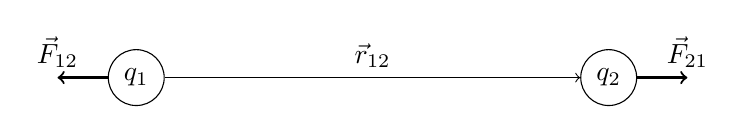
\begin{tikzpicture}
    \path (-3,0) node[draw,circle] (q1) {$q_1$};
    \path (3,0) node[draw, circle] (q2) {$q_2$};
    \draw [->] (q1) -- (q2);
    \draw [thick,->] (q1) -- (-4,0);
    \draw [thick,->] (q2) -- (4,0);
    \node[above] at (0,0) {$\vec{r}_{12}$};
    \node[above] at (-4,0) {$\vec{F}_{12}$};
    \node[above] at (4,0) {$\vec{F}_{21}$};
\end{tikzpicture}
